\subsection{Simulating neural activity in a neural population} \label{sec:results:simulations}

To test the described method for inferring functional connectivity from calcium imaging data, we simulated a network of stochastically connected neurons constructed as close as possible to resemble the real cortical microcircuits, based on experimental data available from the literature \cite{Braitenberg1998, Urquijo2000, Lefort2009, Sayer1990}.  We prepared sparse random networks of $N=10-500$ neurons. Each neuron was modeled using Eqs. \eqref{eqn:glm:definition} and \eqref{eqn:h:definition}.

The network was divided into excitatory (80\%) and inhibitory (20\%) neurons \cite{Braitenberg1998, Urquijo2000}, each respecting Dale's law, i.e., all axons for a particular neuron were either excitatory or inhibitory (corresponding to all positive or all negative columns in our functional connection weight matrix, $\bw$). Neurons were randomly connected to each other with probability $0.1$ \cite{Braitenberg1998, Lefort2009} XXX this isn't strictly true, is it? XXX.  Synaptic weights for excitatory connections, as defined by EPSP peak amplitude, were randomly drawn from exponential distribution with the mean of $0.5 \mu V$ \cite{Lefort2009, Sayer1990}. These were then converted to GLM weights: while synaptic weights physiologically were measured in $\mu V$, in GLM functional connectivity weights were measured in log-rate units of Eq. \eqref{eqn:glm:definition}). GLM weights described the change in the probability of the neuron $i$ to fire given neuron $j$ had fired before, as opposed to physiologically measured injected currents or changes in membrane potential. By utilizing this definition, synaptic weights were converted into GLM weights assuming that each EPSP corresponded to added probability of neuron spiking in given time bin of $\Delta P = V_E/V_{b}$, where $v_E$ is peak EPSP amplitude and $V_b$ is the membrane resting potential below threshold (implying that $V_{b}/V_E$ EPSPs would be required to trigger neuron over the threshold), 

\begin{equation}\label{eqn:convert}
\w_{ij}=\ln(-\ln(e^{-r_i\tau_w}-V_E/V_{b})/r_i\tau_w), 
\end{equation}

\noindent where $r_i=\exp(b_i)$ is the base firing rate of neuron $i$ and $\tau_w=10$ msec was the typical EPSP/IPSP scale over which single EPSP affects the firing probability of the neuron $i$.  %For small $r_i\tau_w$ this could be replaced with
% 
% \begin{equation}\label{eqn:convert-smalldt}
% \w_{ij}=\ln\left(1+\frac{V_E/V_{b}}{r_i\tau_w}\right).
% \end{equation}

Inhibitory connections were also drawn from exponential distribution with the negative mean. Inhibitory connections strength was chosen so as to balance excitatory and inhibitory currents in the network and achieve an average firing rate of  $\approx 5 $ Hz. Practically, the mean strength of inhibitory connections was about 10 times larger than that of the excitatory connections. 

The time course of functional connectivity weights $\w_{ij}(t)$ was modeled as the difference of two exponentials with the rise time of 1 msec and decay time of 10 msec for excitatory and 20 msec for inhibitory currents \cite{Sayer1990}. Up to 25\% variation in these time constants could be allowed. We neglected conduction delays, given that the time delay below $\sim 1$ msec expected in local cortical circuit was smaller than the time step of our computer simulation.  Additionally to excitatory and inhibitory currents, each neuron was modeled to have refractory current with the time-course described as an exponential with time constant of 10 ms.

Spike-trains were generated using GLM by simulating network forward in time with the time step of 1 ms.  Given the spike rasters, the fluorescence observations were generated using calcium dynamics model Eq. \eqref{eqn:ca:definition}. Parameters for the model were chosen according to our experience with few actual cells analyzed using algorithm of \cite{Vogelstein2009}, see Table \ref{table:caparm}.  The population of cells was generated with these parameters allowing cell-to-cell variance of at least 30\%. XXX explain in more detail the distribution from which all the parameters were taken, something like a uniform distribution with bounds based on data.  add to table below the bounds too.  photon budget should be in terms of the actual parameters of our model XXX Fluorescence was obtained for calcium imaging at the frame-rate of 33 Hzor 66Hz.  From 300 sec to 3600 sec of calcium imaging data was simulated.

\begin{table}[h!b!p!]
\caption{Table of simulation parameters.}\label{table:caparm}
\begin{tabular}{ll}
\hline
Total neurons & 10-500 \\
Excitatory neurons & 80\% \\
Connections sparseness & 10\% \\
Baseline firing rate & 5  Hz\\
Mean EPSP strength & 0.5 $\mu$V \\
Mean IPSP strength & 2.3 $\mu$V\\
EPSP profile & 1 msec rise time, 10 msec decay time \\
IPSP profile & 1 msec rise, 20 msec decay time \\
\hline
Mean Ca noise $\sigma_c$ & 28 $\mu$M \\
Mean Ca jump $A_c$ & 80 $\mu$M \\
Mean Ca background $C_b$ & 24 $\mu$M \\
Mean Ca decay time $\tau_c$ & 0.25 sec \\
Mean photon budget $\alpha_c$ & 1-80 Kph/neuron/frame \\
$K_d$ & 200 $\mu$M \\
\hline
\end{tabular}
\end{table}





\begin{figure}[h]
\centering
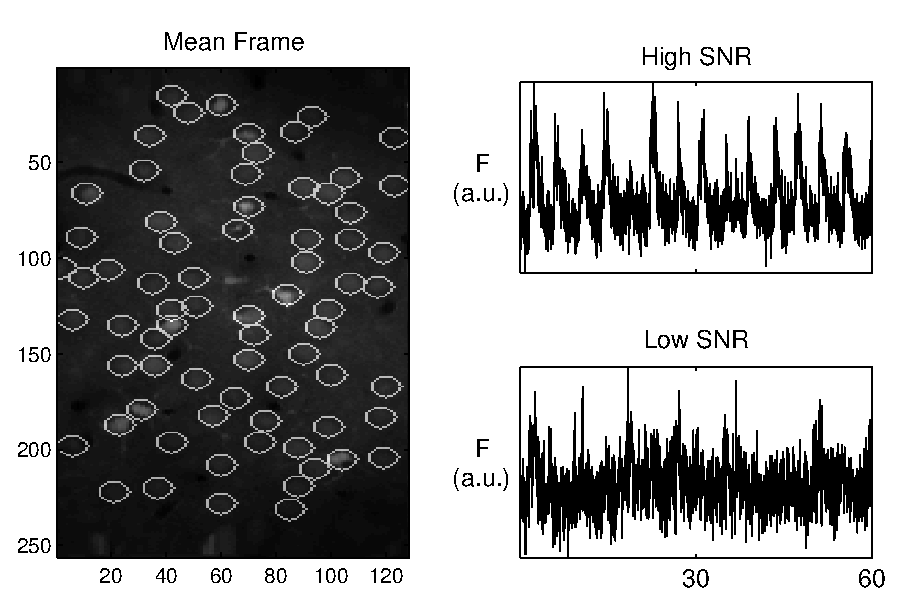
\includegraphics[width=\hsize]{../figs/data_example}
\caption{A schematic depicting our data analysis pipeline.  The left panel shows the mean image from an in vivo experiment, with regions-of-interest indicated by white circles, as determined by a custom algorithm (see Methods for details).  By averaging the pixel intensity of all the pixels within a region of interest, we obtain a one-dimensional fluorescence trace for each neuron.  The middle panel shows two such examples, the top showing a trace with relatively high signal-to-noise ratio (SNR), and the bottom showing a trace with a relatively low SNR.  We use these signals to sample likely spike trains (below each trace), and use such joint spike trains to estimate the functional connectivity matrix, as shown in the left panel.}
\label{fig:data_example}
\end{figure}

% \begin{figure}
% \centering
% \begin{minipage}[c]{0.49\hsize}
% 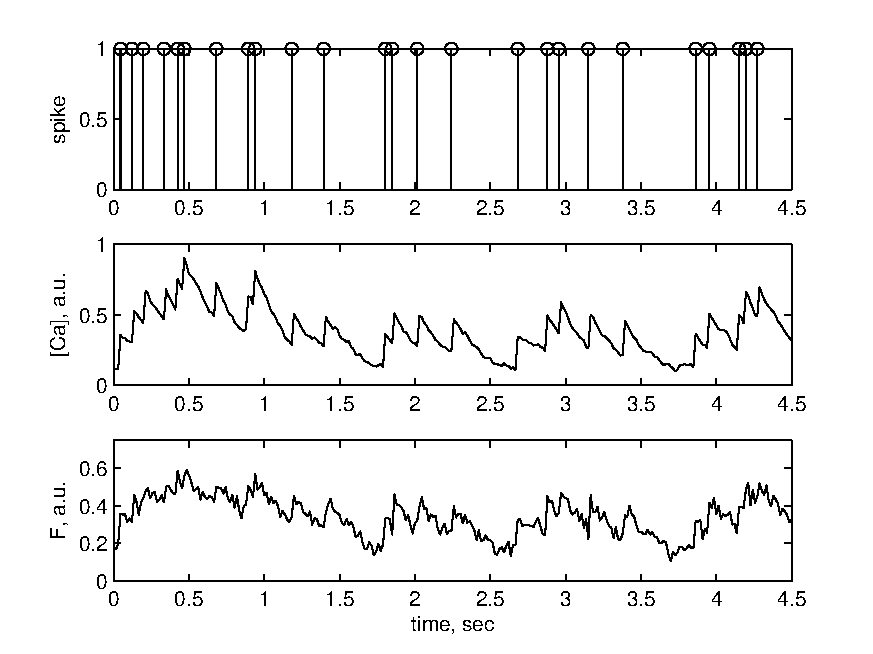
\includegraphics[width=\hsize]{../figs/Figure0b_fluor_eg_hlowSNR}
% \end{minipage}
% \begin{minipage}[c]{0.49\hsize}
% 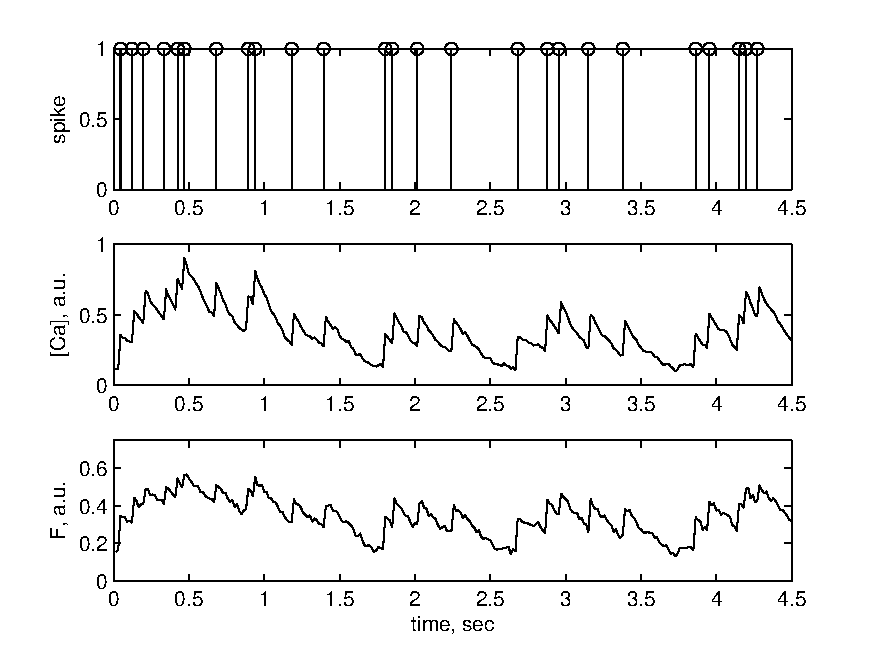
\includegraphics[width=\hsize]{../figs/Figure0a_fluor_eg_highSNR}
% \end{minipage}
% \caption{Examples of calcium and fluorescence traces for low (photon budget 5 Kph/neuron/frame, left)
% and high SNR regimes (photon budget 40 Kph/neuron/frame, right). XXX J will modify to have real data. XXX}
% \label{fig:egfluor}
% \end{figure}

\subsection{Inference of the functional connectivity from the simulated calcium imaging data} \label{sec:results:inference}

\clearpage
\subsubsection{Main Result}

\begin{figure}[h]
%\centering \includegraphics[width=\hsize]{../figs/weights}
\caption{Estimating the functional connectivity matrix. Left: true $\bw$.  Right: estimated $\bw$.  XXX J will make this fig XXX}
\label{fig:w}
\end{figure}

\clearpage
\subsubsection{Time discretization bias}

\begin{figure}[h]
\centering
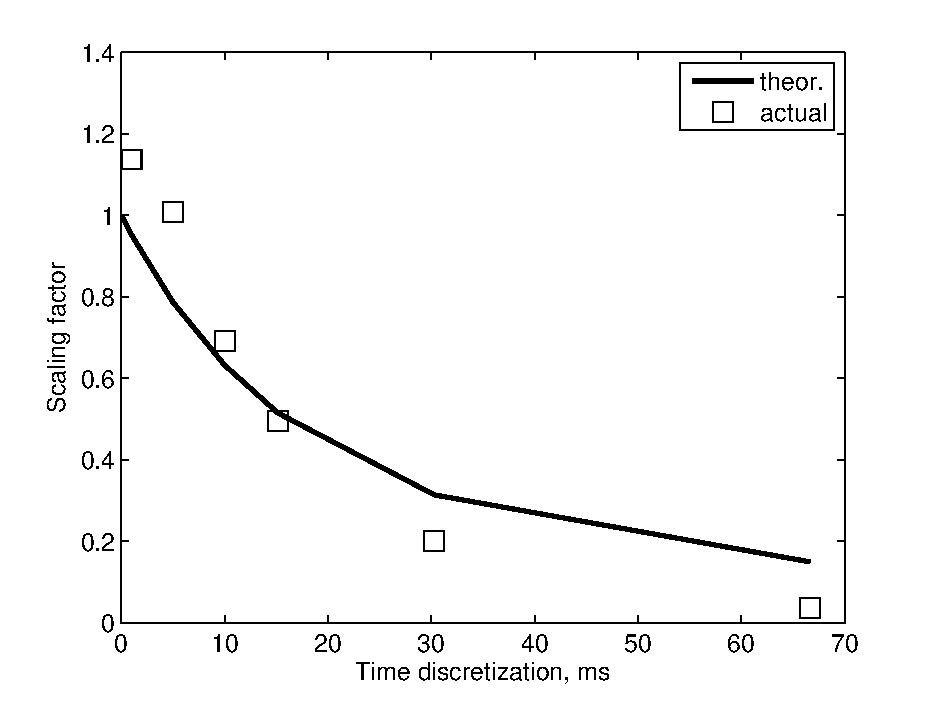
\includegraphics[width=3in]{../figs/Figure13_scalebiasvsframerate}
\caption{We can estimate $W$, but there is some (explainable) bias.}
\label{fig:bias}
\end{figure}

\clearpage
\subsubsection{Inferring weights using $F$}

\begin{figure}[h]
\centering
\begin{minipage}[c]{0.45\hsize}
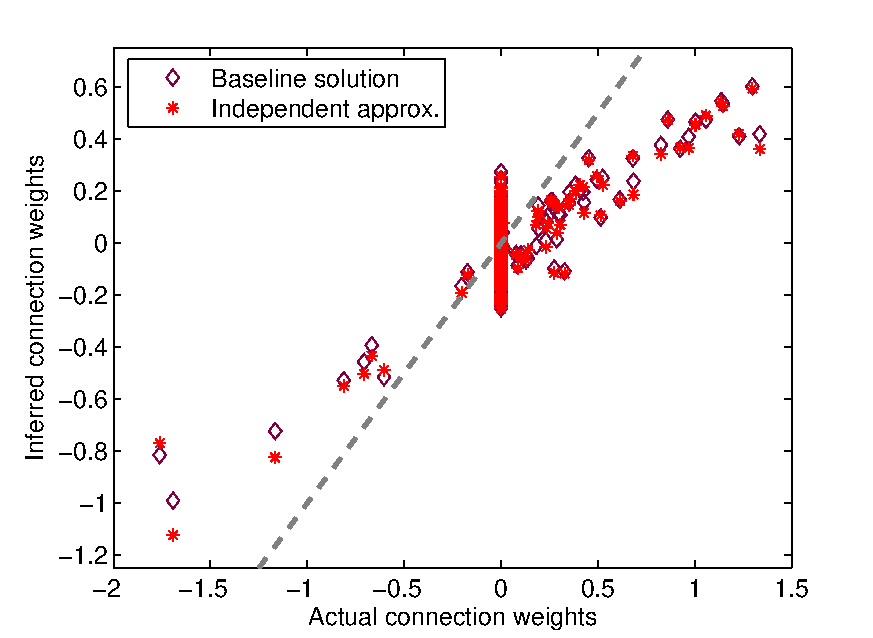
\includegraphics[width=\hsize]{../figs/Figure2_fluor_base_vs_iid}
\end{minipage}
\begin{minipage}[c]{0.45\hsize}
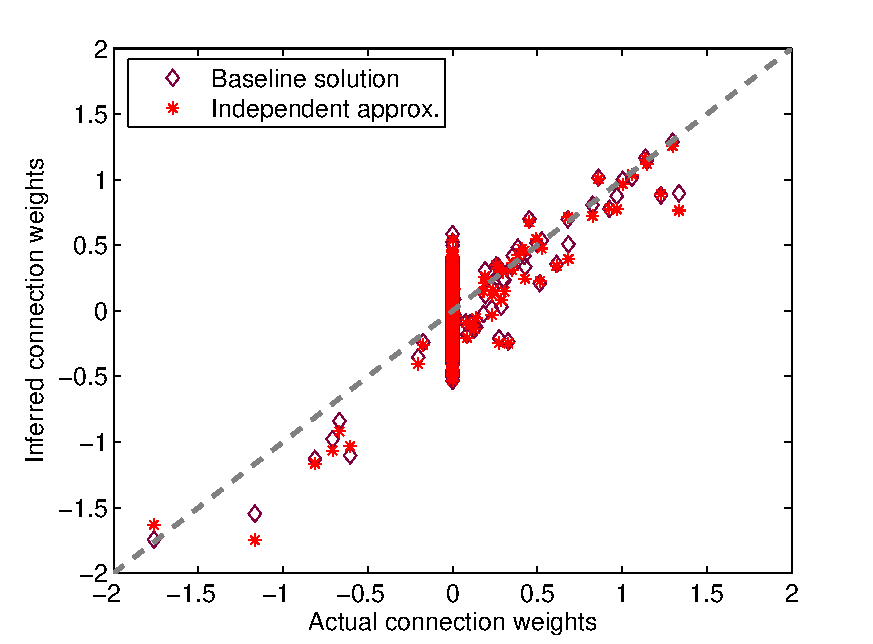
\includegraphics[width=\hsize]{../figs/Figure2b_fluor_base_vs_iid}
\end{minipage}
\caption{A scatter plot of inferred connectivity weights vs. real connectivity weights using independent approximation and true spike trains down-sampled to the frame-rate, for a network of $N=25$ neurons imaged with high SNR (40 Kph/neuron/frame, see Figure \ref{fig:ca-noise} below); $r^2=0.57$ for IID and $r^2=0.57$ for the baseline. Note that for sufficient SNR, the connectivity weights inferred from fluorescence data are nearly equal to such inferred from down-sampled true spikes, thus showing that calcium imaging is capable of achieving accuracy of spike extraction equivalent to direct observation of spike trains. Left panel is the original GLM solution with scaling-bias, and right panel is scaling-bias adjusted solution.  XXX Left panels for these figs i think are great.  perhaps right panels would be more informative if they plotted the biased corrected distributions, as in Figure5-hist-glm-vanilla? XXX}
\label{fig:iid-base}
\end{figure}

\clearpage
\subsubsection{SNR limitations of inferring weights using $F$}

\begin{figure}[h]
\centering 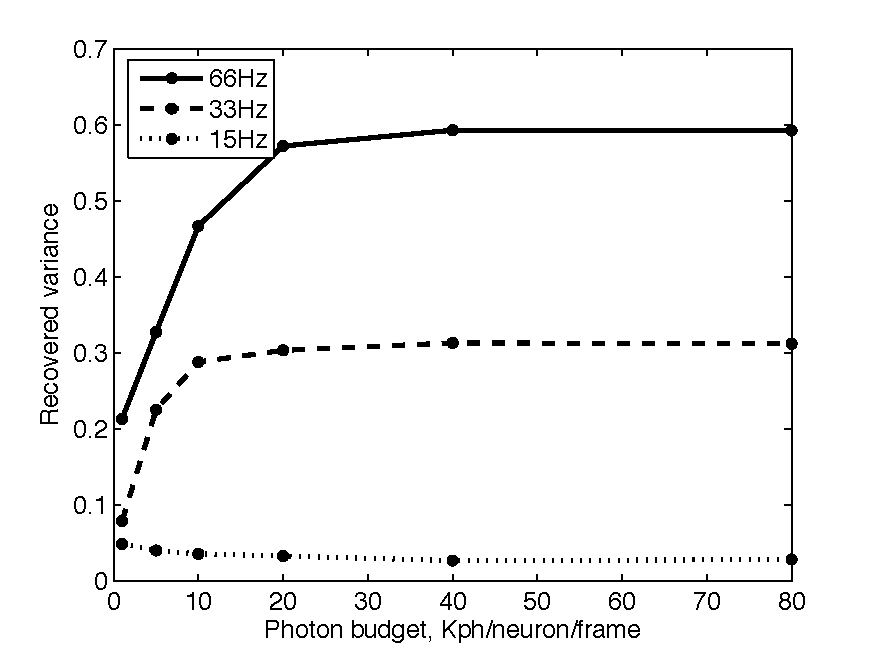
\includegraphics[width=4in]{../figs/Figure4_r2vsSNR}
\caption{$r^2$ as a function of SNR for various FR. XXX Y: did you upload/email that fig? XXX}
\label{fig:snr}
\end{figure}

\clearpage
\subsubsection{Error indep of $N$}

\begin{figure}[h]
\centering
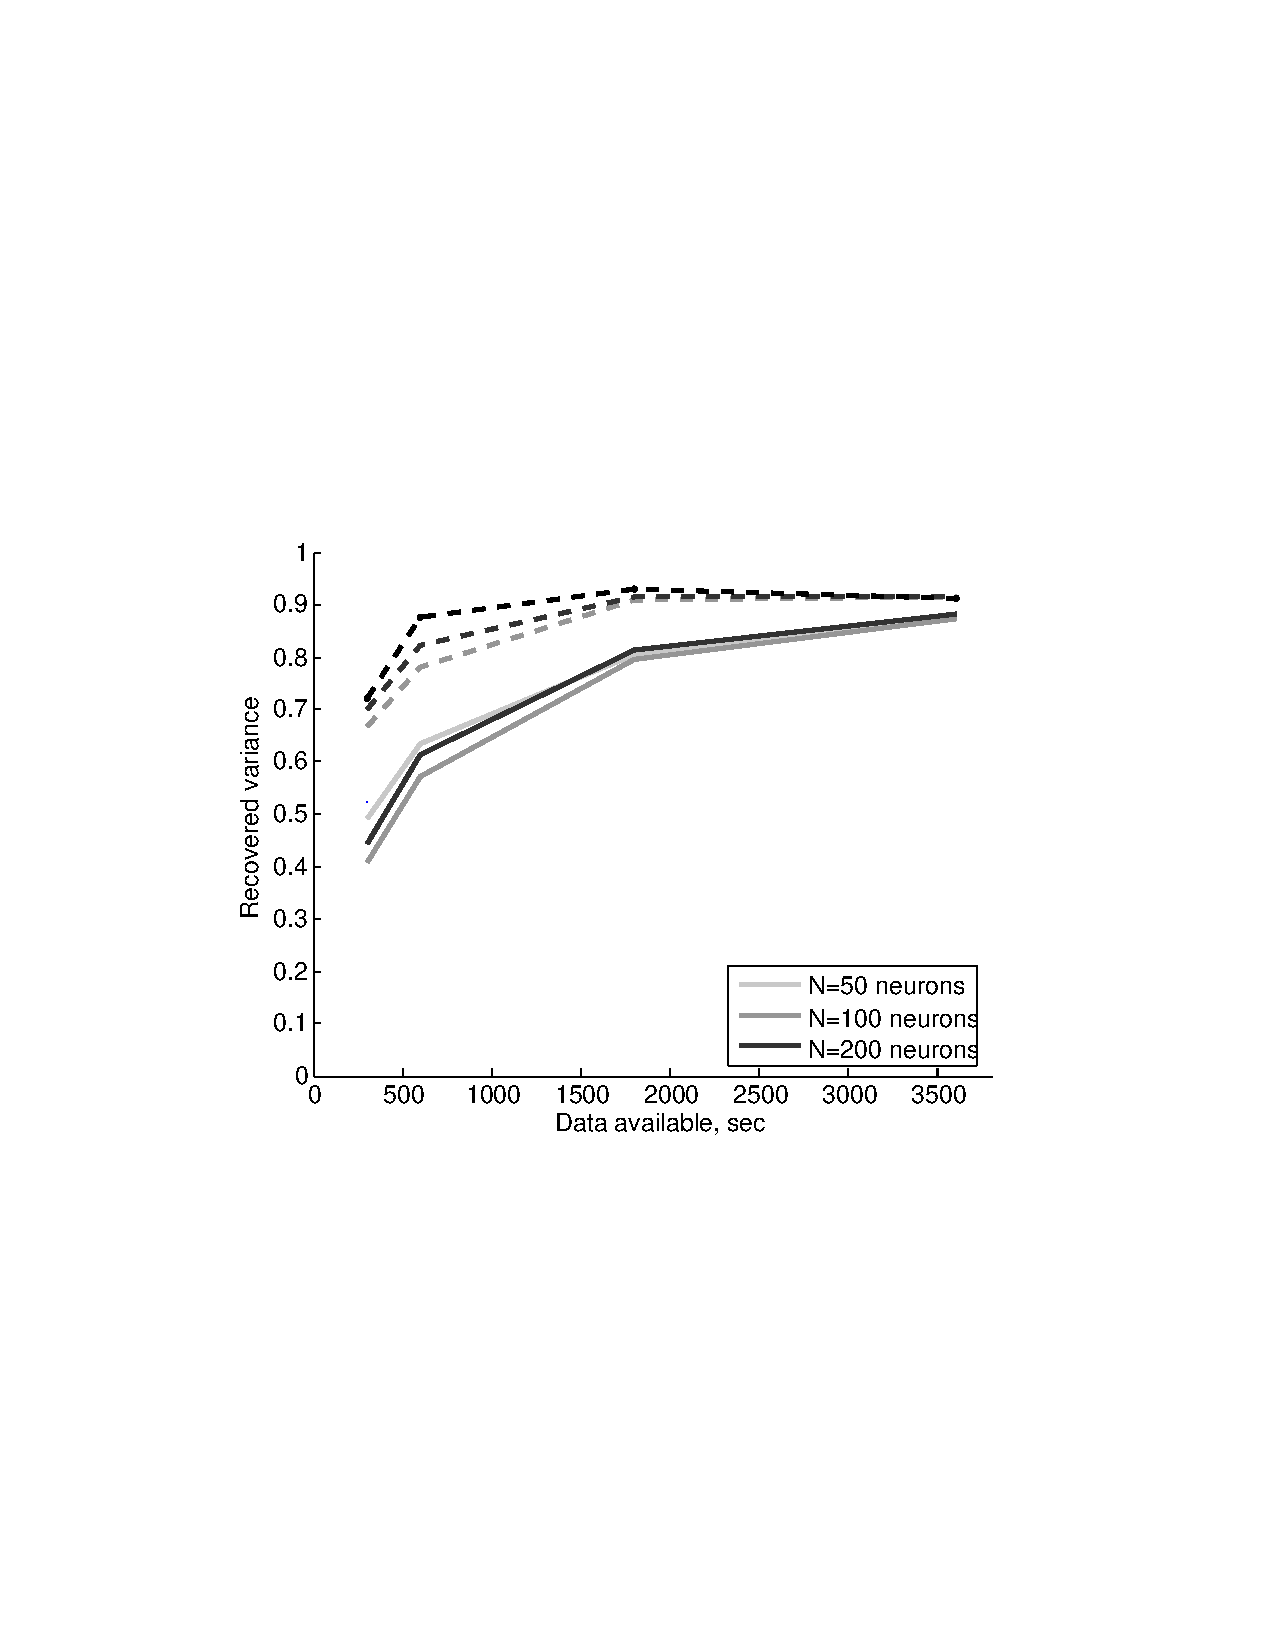
\includegraphics[width=250pt]{../figs/Figure6c_perf_vs_N}
\caption{Baseline accuracy of connectivity weights inference for networks of different size from $N=10$ to $N=200$ neurons. Accuracy does not depend on the number of neurons $N$ in agreement with theoretical analysis in Methods. 300-600 seconds of calcium imaging data are sufficient for estimating connectivity matrix using sparse-prior GLM solver, and about 30 minutes of observations are sufficient using GLM solver. XXX  does it make sense to include the sparse solutions in this fig, given that we haven't introduced them yet? XXX}
\label{fig:data-n}
\end{figure}


\clearpage
\subsubsection{Correlations kill estimates}

\begin{figure}[h]
\centering
\begin{minipage}[c]{0.45\hsize}
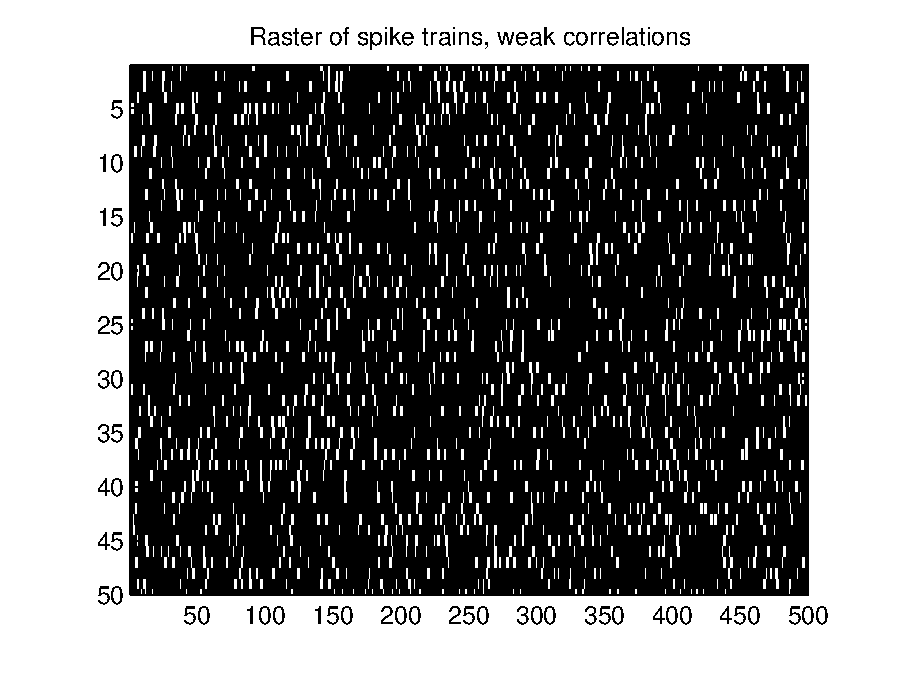
\includegraphics[width=\hsize]{../figs/Figure7b_raster_weak}
\end{minipage}
\begin{minipage}[c]{0.45\hsize}
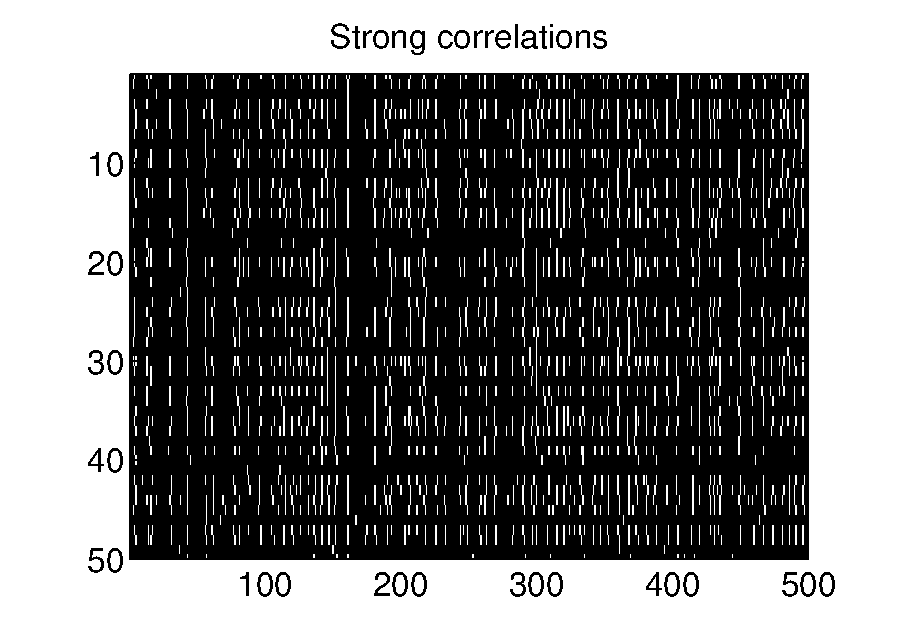
\includegraphics[width=\hsize]{../figs/Figure7a_raster_strong}
\end{minipage}
\begin{minipage}[c]{0.45\hsize}
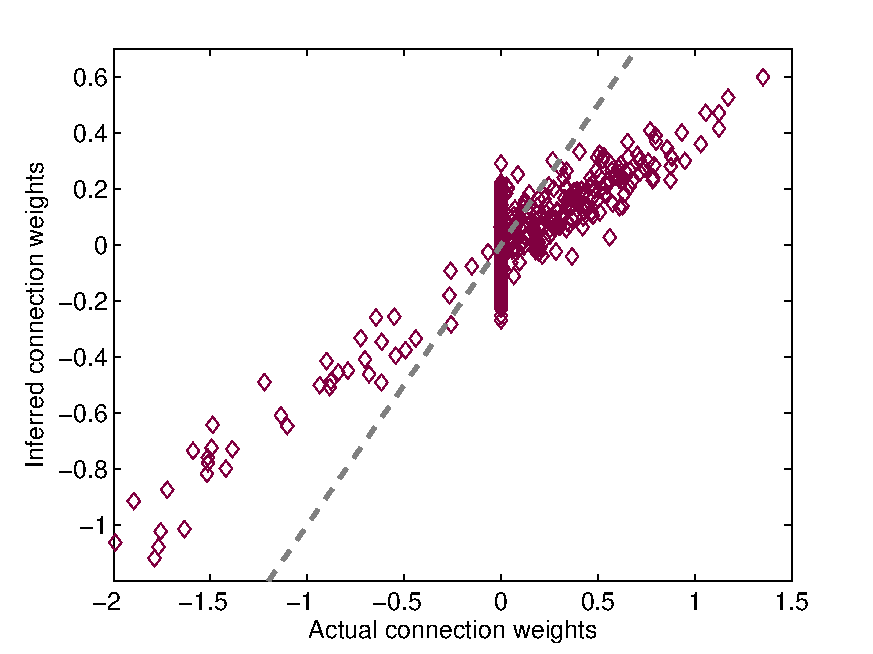
\includegraphics[width=\hsize]{../figs/Figure8b_fluor_weak_glm}
\end{minipage}
\begin{minipage}[c]{0.45\hsize}
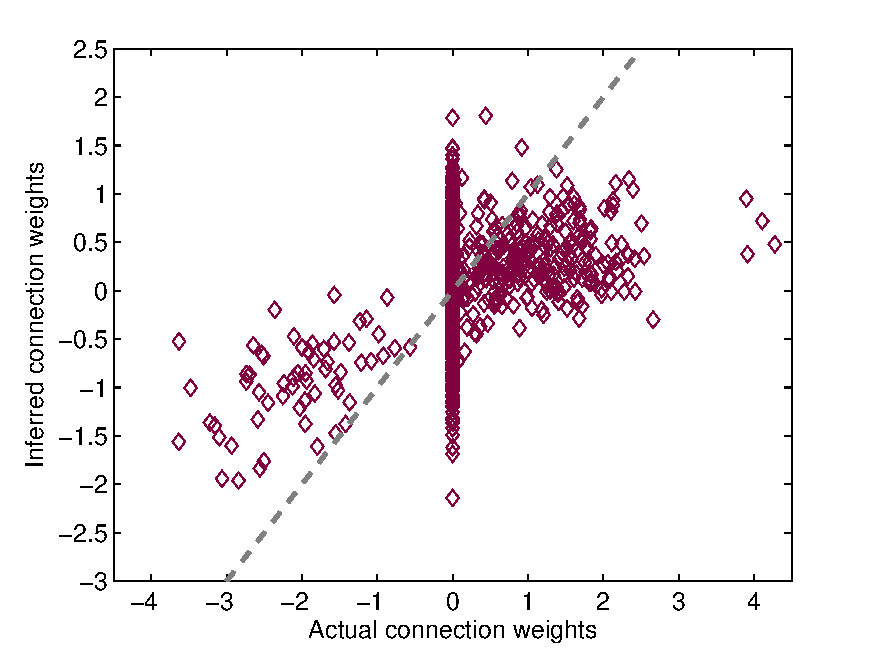
\includegraphics[width=\hsize]{../figs/Figure8a_fluor_strong_glm}
\end{minipage}
\caption{15 sec of simulated spike trains for a weakly coupled (upper-left)
and strongly coupled (upper-right) stochastic networks. Note that in weakly coupled network spikes are sufficiently uncorrelated to allow access to all different neural connectivity configurations necessary to estimate complete anatomical connectivity vectors ${\bf w}_i$. In strongly coupled case many instances of highly synchronous locked firings are evident, thus reducing dimensionality of the observed dynamic space of the network, and preventing functional connectivity from faithfully representing anatomical connectivity.
Accordingly, GLM solution for strongly coupled neural network (lower-right) does not provide access to the structure of anatomical connectivity as opposed to weakly-coupled case (lower-left).  XXX maybe a third row showing the distributions? XXX}
\label{fig:rasters}
\end{figure}

\clearpage
\subsubsection{Robustness to variability in $\tau_h$}

\begin{figure}[h]
\centering
\begin{minipage}[c]{0.45\hsize}
%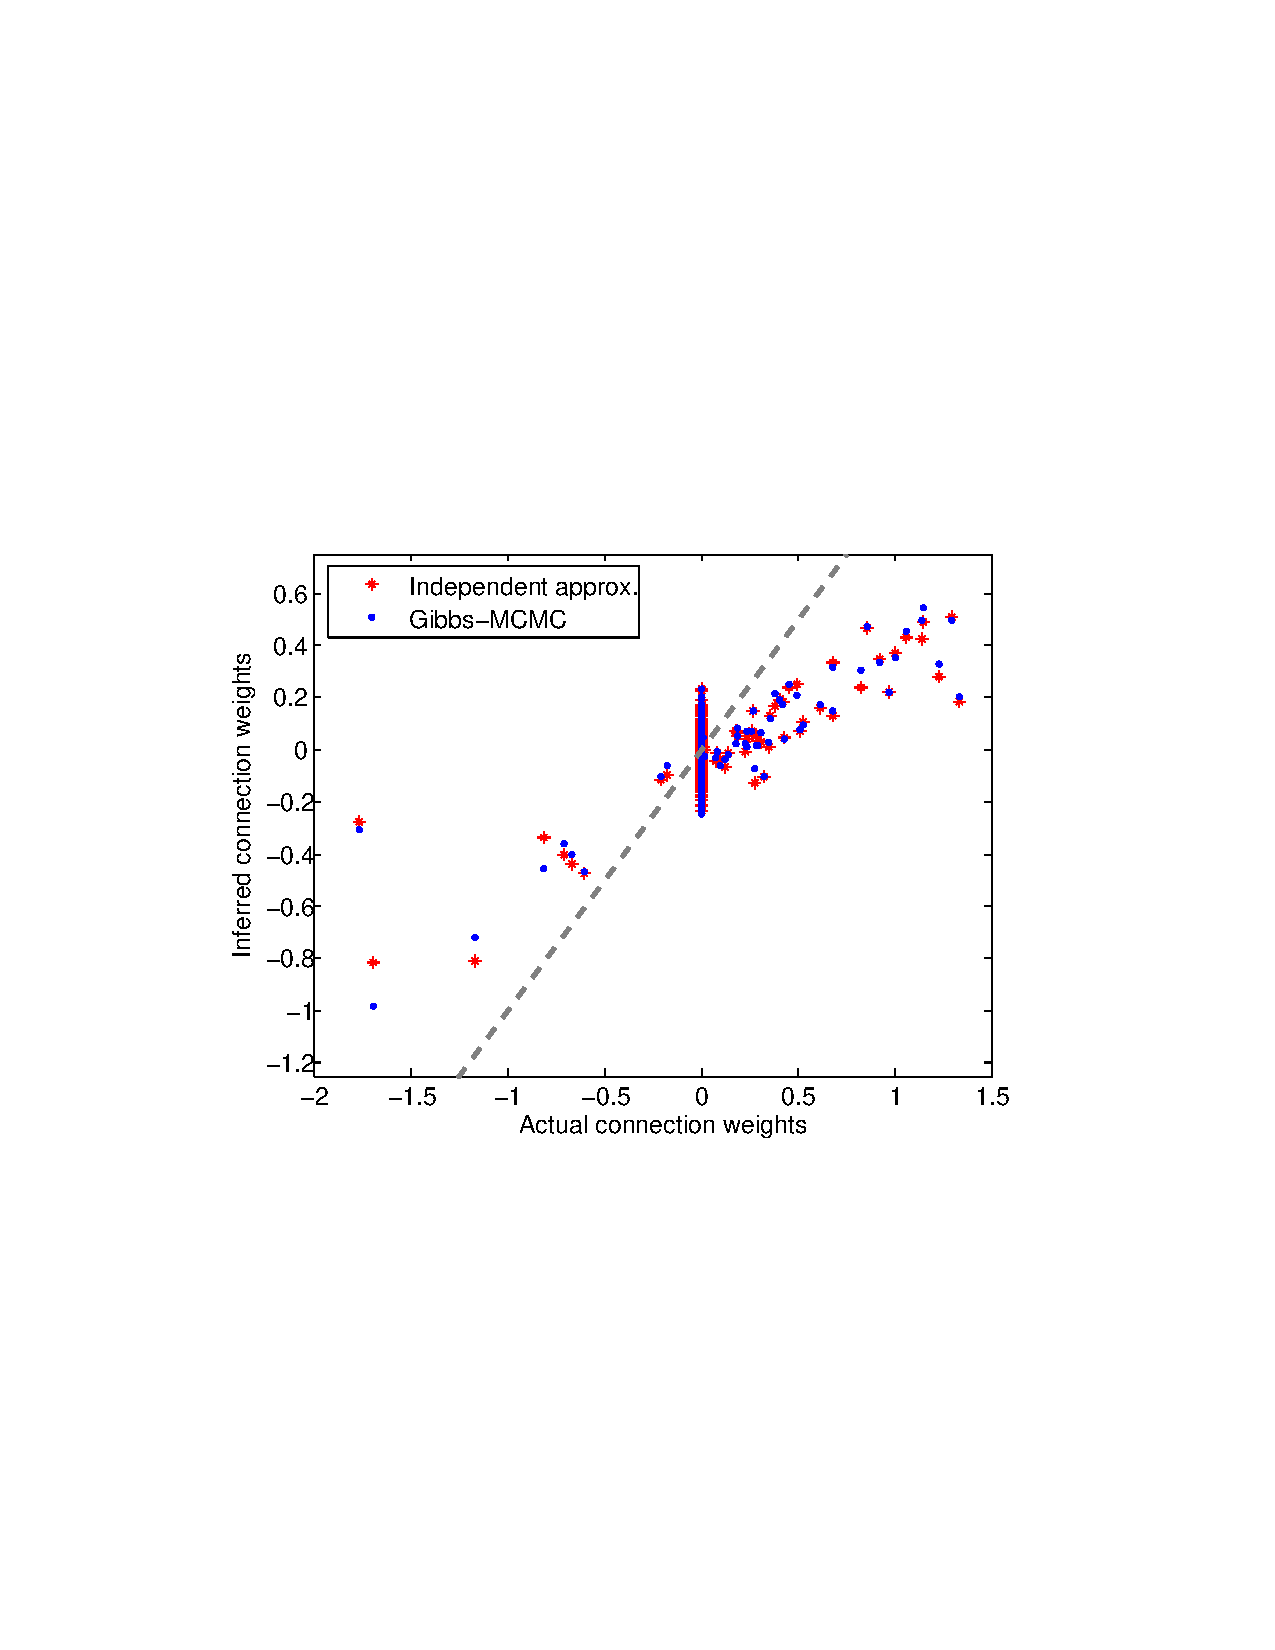
\includegraphics[width=\hsize]{../figs/Figure1_fluor_mcmc_vs_iid}
\end{minipage}
\begin{minipage}[c]{0.45\hsize}
%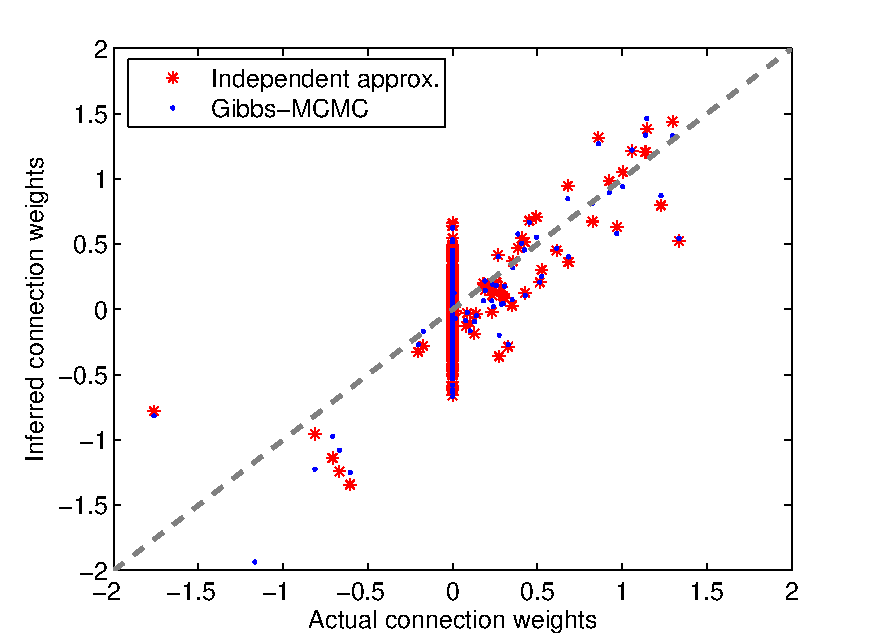
\includegraphics[width=\hsize]{../figs/Figure1b_fluor_mcmc_vs_iid}
\end{minipage}
\caption{something like fig 4 for Robustness to variability in $\tau_h$}
\label{fig:mcmc-iid}
\end{figure}

\clearpage
\subsubsection{Hybrid MCMC-Gibbs outperforms indep approx}

\begin{figure}[h]
\centering
\begin{minipage}[c]{0.45\hsize}
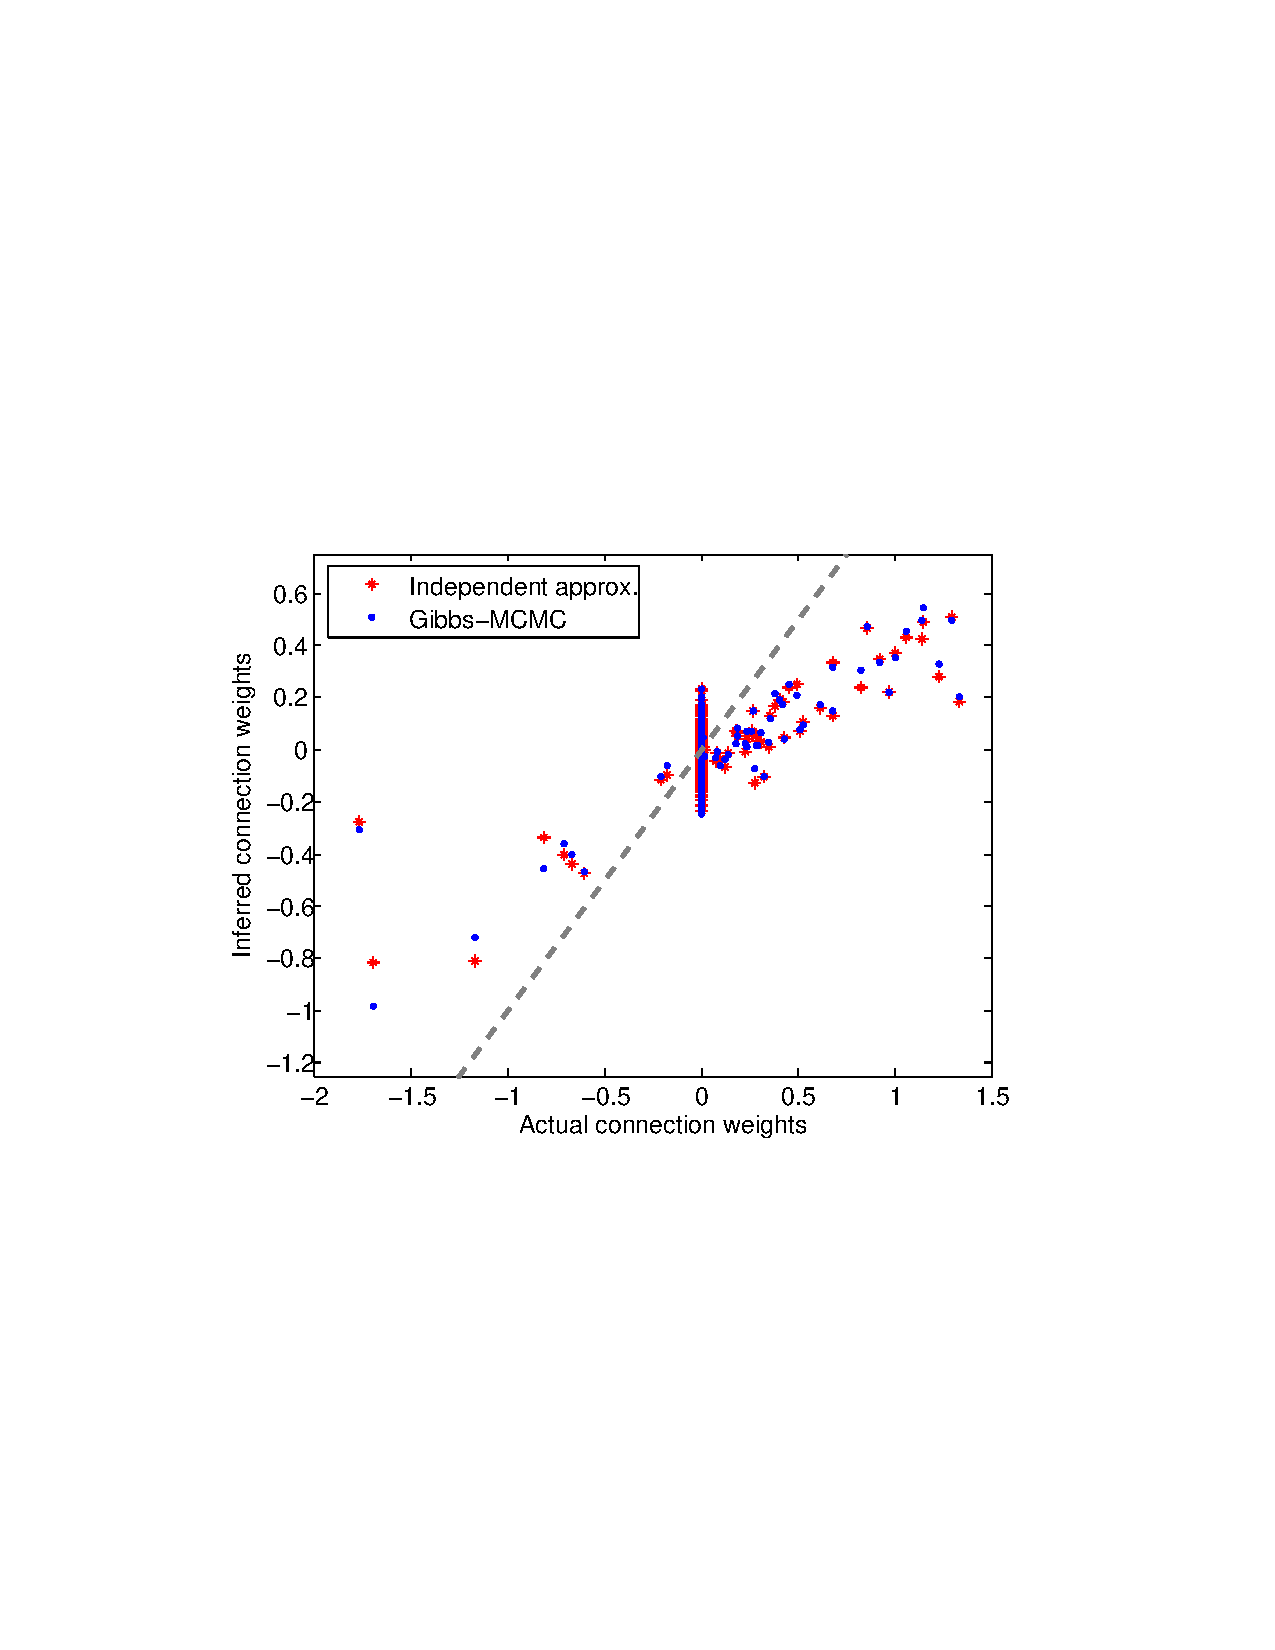
\includegraphics[width=\hsize]{../figs/Figure1_fluor_mcmc_vs_iid}
\end{minipage}
\begin{minipage}[c]{0.45\hsize}
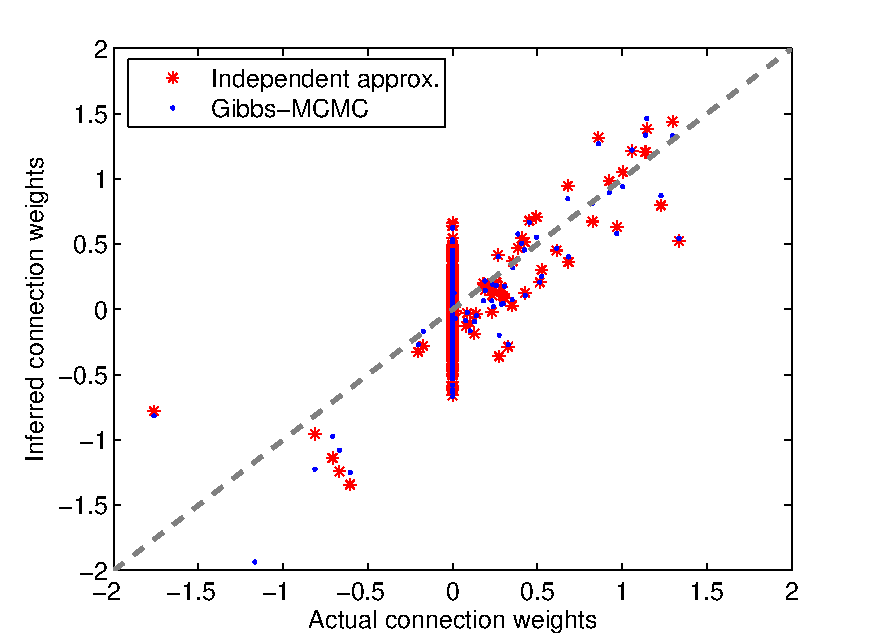
\includegraphics[width=\hsize]{../figs/Figure1b_fluor_mcmc_vs_iid}
\end{minipage}
\caption{A scatter plot of inferred connectivity weights vs. real connectivity weights
using hybrid MCMC-Gibbs sampler and independent approximation, for a network of $N=25$ neurons imaged
with intermediate SNR ($10$ Kph/neuron/frame, see Figure \ref{fig:ca-noise} below); $r^2=0.48$ for MCMC-Gibbs and
$r^2=0.47$ for IID. Note that the connectivity weights thus inferred are nearly equal, thus showing that independent approximation is sufficient here for the purposes of estimating the connectivity matrix. Note also constant time-discretization scaling bias in the estimated weights due to missing proximal spike pairs (left panel). 
Scaling-bias adjusted weights correspond to true connectivity weights well (right panel). XXX same comment as fig 4 XXX}
\label{fig:mcmc-iid}
\end{figure}

\clearpage
\subsubsection{Sparse prior improves estimate}

\begin{figure}[h]
\centering
\begin{minipage}[c]{0.45\hsize}
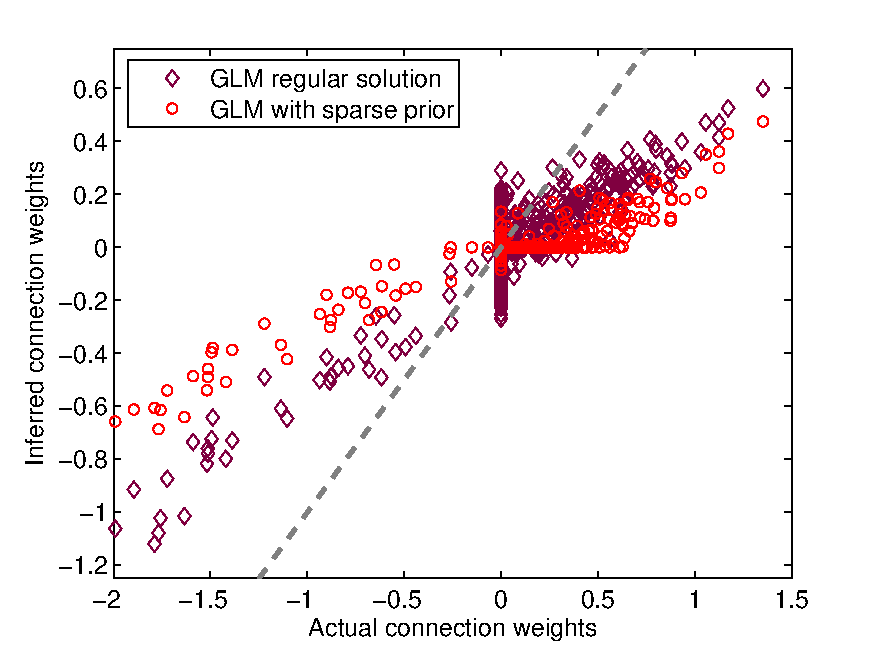
\includegraphics[width=\hsize]{../figs/Figure9_fluor_sparse_sol}
\end{minipage}
\begin{minipage}[c]{0.45\hsize}
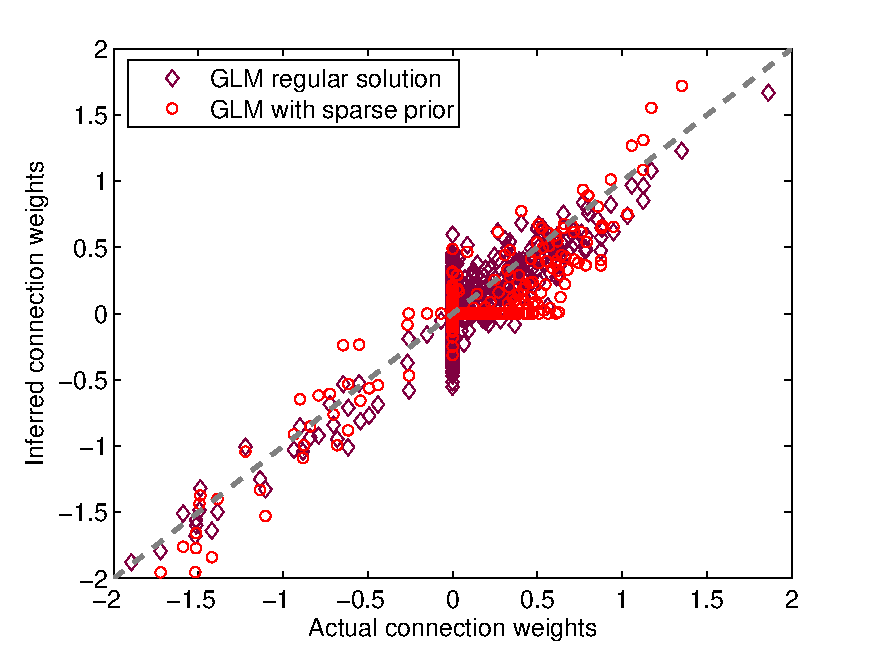
\includegraphics[width=\hsize]{../figs/Figure9b_fluor_sparse_sol}
\end{minipage}
\caption{A scatter plot of inferred connectivity weights vs. real connectivity weights
using independent approximation and either GLM or sparse-prior GLM,
for a network of $N=50$ neurons imaged for $T=800$ s
with high SNR (40 Kph/neuron/frame, see Figure \ref{fig:ca-noise} below); $r^2=0.66$ for GLM solution and $r^2=0.85$ for sparse-prior GLM solution. Note that use of sparse prior allows to obtain significantly better approximation to the true connectivity matrix, although additional scaling bias is introduced in the estimate.
Left panel is the original GLM solution with scaling-bias, and right panel is scaling-bias adjusted solution. XXX same comment as fig 4 XXX}
\label{fig:sparse-sol}
\end{figure}


\clearpage
\subsubsection{Other}

Connectivity matrix was calculated by solving maximum likelihood problem Eq. \eqref{eqn:likelihoodGLM-expl}. Specifically, 

\begin{align}
\label{eqn:likelihoodGLMmoda}&E[\ln P_{\bn}(n_i|{\bf n}_{\i}; W)]=\sum_t \left( n_i(t) \ln J_i(t) - (1-n_i(t)) \exp(J_i(t)) \Delta \right), \\
\label{eqn:likelihoodGLMmodb}&J_i(t)=b_i+\sum\limits_j \sum\limits_{t'<t} \w_{ij}(t-t')n_{j}(t')=
b_i+\sum\limits_j w^{ij}_s \sum\limits_{t'<t} \exp(-(t-t')/\tau_h)n_j(t').
\end{align}

The sum in Eqs.\eqref{eqn:likelihoodGLMmoda} and \eqref{eqn:likelihoodGLMmodb} was over the sample of $\{n_i(t)\}$ and over the time-bins $t'$ discretized at the time steps $\Delta$ corresponding to the calcium imaging frame rates of either 33 Hz (30 ms) or 66 Hz (15 ms). The coincident time bin $t=t'$ was not used in Eqs.\eqref{eqn:likelihoodGLMmoda}), \eqref{eqn:likelihoodGLMmodb}), i.e.  all spike pairs within same time-frame were removed from the GLM fit.  Because time position of spikes inferred from fluorescence data typically had inaccuracy $\sim \Delta$, temporal order of such closely positioned spike pairs could be confused in the sample ${\bf n}$, thus, polluting GLM dataset.  E.g., given two neurons $i$ and $j$, if the number of spikes of neuron $i$ following neuron $j$ within $\Delta$ was $m_{ij}$, while such in the reverse order was $m_{ji}$, the difference $\Delta m = m_{ij}-m_{ji}$ effectively corresponded to the difference in GLM weights $\w_{ij}-\w_{ji}$. However, if during spike inference the order of such spikes was confused with probability $p\approx 1/2$, the observed number of spike pairs $ij$ would become $m_{ij}(1-p)+m_{ji}p$, while for the reverse order this would be $m_{ji}(1-p)+m_{ij}p$. The difference would thus drop to $\Delta m '= (1-2p)\Delta m$ with the variance remaining the same. This effect complicated the problem of estimating functional connectivity $W$ by effectively mixing $\w_{ij}$ and $\w_{ji}$ and introducing large error in $W$ estimate moving it toward the symmetrized version of $W$.

Since the connectivity weights $\w_{ij}(t)$ were time-dependent, to compare inferred and true connectivity we introduced a ``scalar'' version of the connectivity matrix defined via the peak values of EPSP/IPSP at each connection, i.e. the scalar connection weights were $w^{ij}_s=\text{sign}(\w_{ij})\max_{t} |\w_{ij}(t)|$.  If the time dependence of $\w_{ij}(t)$ was assumed to be unknown, the first equation in \eqref{eqn:likelihoodGLMmodb}) was used to correlate $n_i(t)$ with $n_j(t')$ for $t'<t$ up to given depth $m$.  Since each next term in Eq. \eqref{eqn:likelihoodGLMmodb}) was exponentially smaller than the previous one, we found that the best results were obtained assuming $m=1$, allowing for better results by reducing the number of unknowns for the same amount of data.  For independent approximation below the time-dependence of $\w_{ij}(t)$ was assumed to be `'known'' exponential, and the weights were estimated using reduced histories $h_{i}(t)=\sum_{t'<t} \exp(-(t-t')/\tau_h)n_{i}(t')$ with time constant $\tau_h=10$ ms. The scalar connection weights were directly estimated as $w^{ij}_s=\w_{ij}(t=0)$.  Such inferred connectivity weights were then compared with true $w^{ij}_s$.

We shall note that because of coarse time discretization $\Delta \approx 15-30$ msec relative to EPSP/IPSP time scale of $\tau_w = 10-20$ ms, the first term in the sum \eqref{eqn:likelihoodGLMmodb}) measured in GLM was $\w_{ij}(\Delta)\approx w^{ij}_s\exp(-\Delta/\tau_w)$, substantially smaller than $w^{ij}_s$. Time discretization thus resulted in estimated weights differing from the true connectivity by a factor of $\sim \langle \exp(-\Delta/\tau_w) \rangle$, where the average is understood over the spike pairs within two consecutive time-bins. In our simulations, we observed that this factor was a constant for same $\Delta$ and $\tau_w$ and different network sizes $N$. For $\Delta=15$ msec and $\tau_w\approx 10$ msec this factor was  $\approx 0.45$.  Note that where $\tau_w$ varied from neuron to neuron, this scaling factor as well as any mismatch in the time-scale $\tau_h$ of $h_i(t)$ and the true EPSP/IPSP time constant $\tau_w$ introduced added variability in the estimated weights $w^{ij}_s$. However, we found such added variance in the estimates of $w^{ij}_s$ to be insignificant for simulations where $\tau_w$ was allowed to vary for up to 25\% (data not shown).

Scaling bias theoretically could be removed by performing estimation of spike trains with finely discretized time. However, we were not successful in performing this calculation as the amount of data necessary to overcome variation in $W$ introduced by disordering of closely spaced spike-pairs appeared to be well over $\approx 10$ min of data used for most of the calculations here. Such high-time-resolution samples of spike trains were also substantially more computationally expensive to obtain and work with. For these reasons we did not pursue this path further, although it may be of interest in the future.

After performing functional connectivity reconstruction using MCMC-Gibbs method, we repeated the reconstruction using independent approximation. We found that MCMC-Gibbs method did not provide noticeable improvement over the independent approximation for imaging regimes where sufficiently accurate connectivity matrix could be recovered, Figure \ref{fig:mcmc-iid}. We therefore concluded that the independent approximation was equivalent to exact MCMC-Gibbs method for the purpose of inferring connectivity from calcium imaging data for experimentally interesting regimes.

Since fluorescence data is generally acquired at low frame-rate, one of the main limitation for the connectivity inference from calcium imaging is time-resolution of the inferred spike trains. In order to determine the limits on reconstruction due to this constraint, we compared weights inferred from fluorescence data with such computed from the true spike trains down-sampled at frame-rate of 33 Hz or 66Hz. This served as a baseline for the ``best'' connectivity matrix reconstructions. We observed that baseline performance could be achieved from calcium imaging data, Figure \ref{fig:iid-base}.  Also, the same analysis of baseline performance showed that calcium imaging rates below 30 Hz are generally insufficient for the purpose of inferring connectivity, Figure XXX.


[ANOTHER FIGURE 30Hz]

We then considered the question what calcium imaging SNR was required to achieve time-resolution performance limits, particularly as determined by the photon budget of the experimental setup. Photon budget is defined here as the average count of photons collected by the detector from single neuron per single frame. It is experimentally determined by the factors such as dye quantum efficiency, excitation laser power, detector efficiency, microscope scanning speed, etc. Photon budget was one of the primary factors determining possibility of analyzing spike trains from calcium imaging data (the other key factors being frame-rate and neuron peak spike rate).  As should be expected, when amount of noise was high (low photon budget), inference from calcium imaging data was far below the baseline level, and with increasing SNR the baseline level was recovered. The SNR level necessary to achieve baseline performance was 20-40 Kph/neuron/frame, Figure \ref{fig:ca-noise}.  For comparison, from our experience with the analysis of real cells \cite{Vogelstein2009}, the photon budget in real data was $\sim 10$ Kph/cell/frame for in-vivo data collected at 15  Hz and $\sim 100$ Kph/cell/frame for in-vitro data at the same frame-rate.

\begin{figure}[h]
	\centering
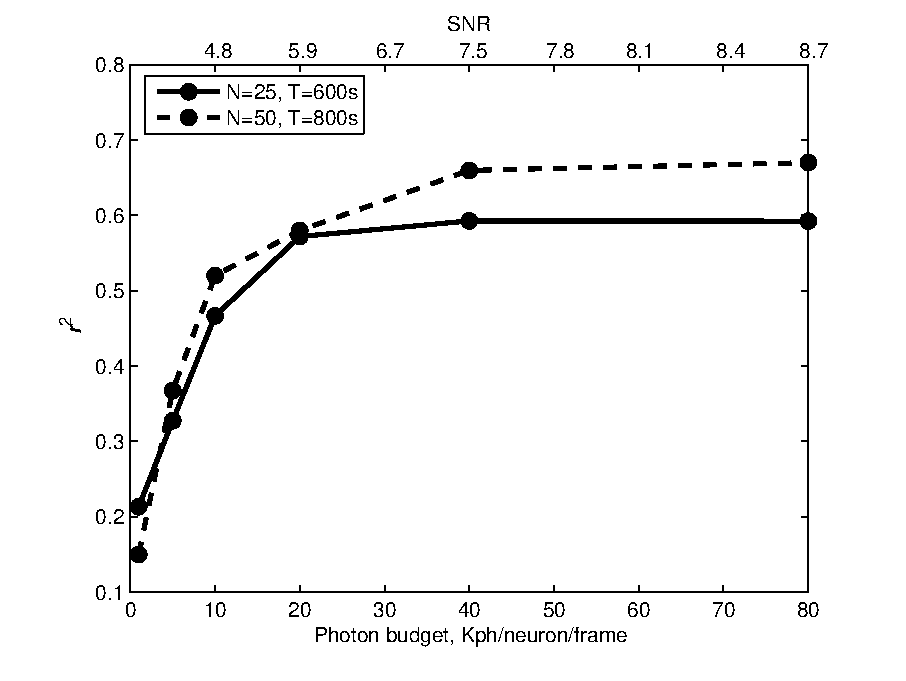
\includegraphics[width=275pt]{../figs/Figure3_perf_vs_gamma}
\caption{Accuracy of inferred connectivity weights as function of noise amount in calcium imaging data, as measured by photon budget per neuron-frame and fluorescence signal to noise ratio SNR=$\left({E[\Delta F^2 | \text{spk}]}/{E[\Delta F^2|\text{nospk}]}\right)^{1/2}$,  for networks of $N=25$ and $N=50$ neurons. Note that the photon counts on the order of 20-40 Kph/frame/neuron are required in order to achieve best reconstructions.}
\label{fig:ca-noise}
\end{figure}

In all cases we found that taking into account sparseness prior resulted in dramatic improvement in the inferred connectivity matrix, allowing to achieve for $T\sim 10$ min the same level of accuracy that would otherwise require over $T\sim 1$ hour of calcium imaging data (Figure \ref{fig:sparse-sol} and \ref{fig:data-time}). We also explored impact of the Dale's prior and found that improvement in the inferred weights there were much less significant, on the order of $10\%$ in the correlation coefficient $r^2$. If sparseness of the solution was previously accounted for, accounting for Dale's law led to no improvement in the result (Figure \ref{fig:data-time}).

We finally explored the question how much data was required for given reconstruction accuracy. First, we considered different observation times $T$, see Figure \ref{fig:data-time}. The observation time necessary to achieve $r^2$=0.5 was $T\sim 10$ minutes, while with GLM solver using sparse prior $r^2>0.6$ was achieved already at $T\sim 5$ minutes of calcium imaging. In agreement with the theoretical analysis of the Fisher information matrix in the Methods, the accuracy of the reconstruction did not depend on the size of the neural network inferred, see Figure \ref{fig:data-n}. Good reconstructions for $N=20-200$ could be obtained in all cases with $T\sim 10-30$ min of data. We conclude therefore that the connectivity could be successfully inferred from calcium imaging data, Figures \ref{fig:sparse-sol}, \ref{fig:distr} and \ref{fig:data-time}).

``Anatomical'' connectivity could be recovered despite potential problems such as common input from correlated neurons, etc. This is owing to the particular form of the activity in our neural network, whereas firing of neurons occurred independently, thus, allowing GLM explore full range of possible input configurations and disentangle potential common inputs.  Estimation of the functional connectivity is fundamentally routed in observing changes in the spike rates conditioned on the state of the other neurons. Intuitively, such estimation can be compared to observing changes in $p({\bf n}(t))=\exp(\sum_j \w_{ij}n_j(t))$ for different neural configurations ${\bf n}(t)$ or, equivalently, estimating vector ${\bf w}_i$ by observing a number of dot-products ${\bf w}_i {\bf n}(t)$ with different vectors ${\bf n}(t)$. Obviously, in order to be able to properly estimate all components of ${\bf w}_i$ the set of available ${\bf n}(t)$ should be rich enough to span all $N$ dimensions of ${\bf w}_i$. In case of independent firing such condition of ``full dimensionality'' is clearly satisfied.  Should this condition be violated, however, e.g. due to high correlation between spiking of few neurons, spike trains will not necessarily provide access to complete anatomical connectivity vector ${\bf w}_i$, and so the connection weights from the neurons providing correlated input may be ``aggregated'' into a single weight, split arbitrarily into a linear combination of weights, etc.

To test this effect we performed simulation of a hypothetical strongly coupled  neural network, still with unstructured random sparse connectivity now consisting additionally of strong component. Strong connections component was chosen to dynamically build up the actual firing rate to $\approx 5$  Hz from the base rate low $r=\exp(b_i)\approx 1$ Hz . Such strongly coupled network showed patterns of firing very different from weakly coupled networks considered above, Figure \ref{fig:rasters}.  In particular, large number of highly correlated, synchronously locked firings of many neurons were evident in this network.  Likewise, GLM was not able to identify the true connectivity matrix correctly, Figure \ref{fig:rasters}. 

\begin{figure}[h]
	\centering
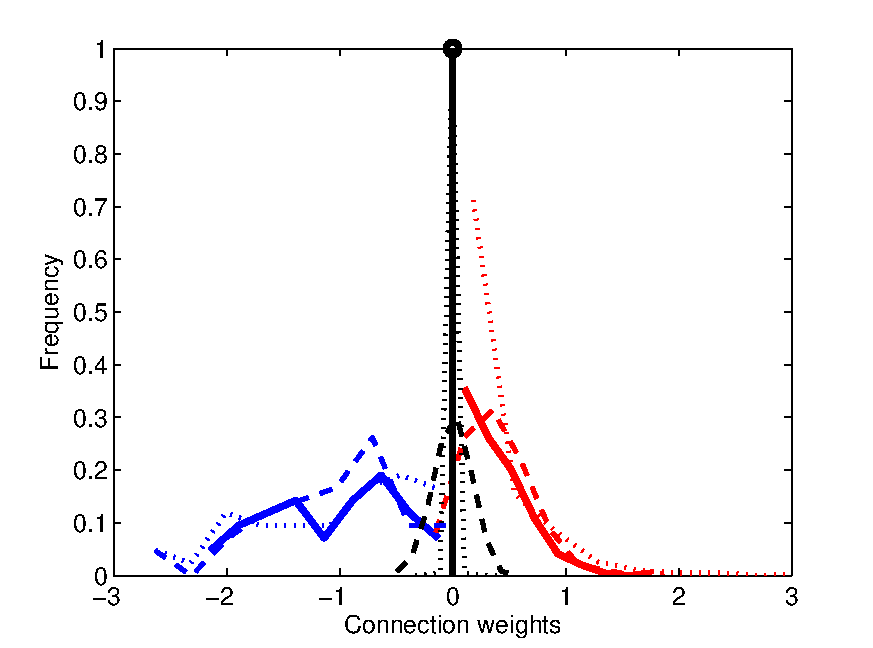
\includegraphics[width=250pt]{../figs/Figure5_hist_glm_vanilla}
\caption{Distribution of connectivity weights inferred using calcium imaging, for a network of $N=50$ neurons and $T=800$ s. The inferred distributions were rescaled to have the same mean with the true distributions, owing the time-discretization scaling bias discussed in the text. Left panel is for GLM solution, and right panel is for sparse-prior GLM solution. Blue curves are for inhibitory connections, red curves are for excitatory connections and black are for zero connections. Solid lines are original distributions and dashed lines are inferred distributions. In GLM solution the quality of the inferred weights is certainly sufficient to say whether a pairs of neurons is connected, or whether given neuron is inhibitory or excitatory with high reliability; and such statements may be made from sparse-prior GLM solution almost with certainty.}
\label{fig:distr}
\end{figure}


\begin{figure}[h]
\centering
\begin{minipage}[c]{0.30\hsize}
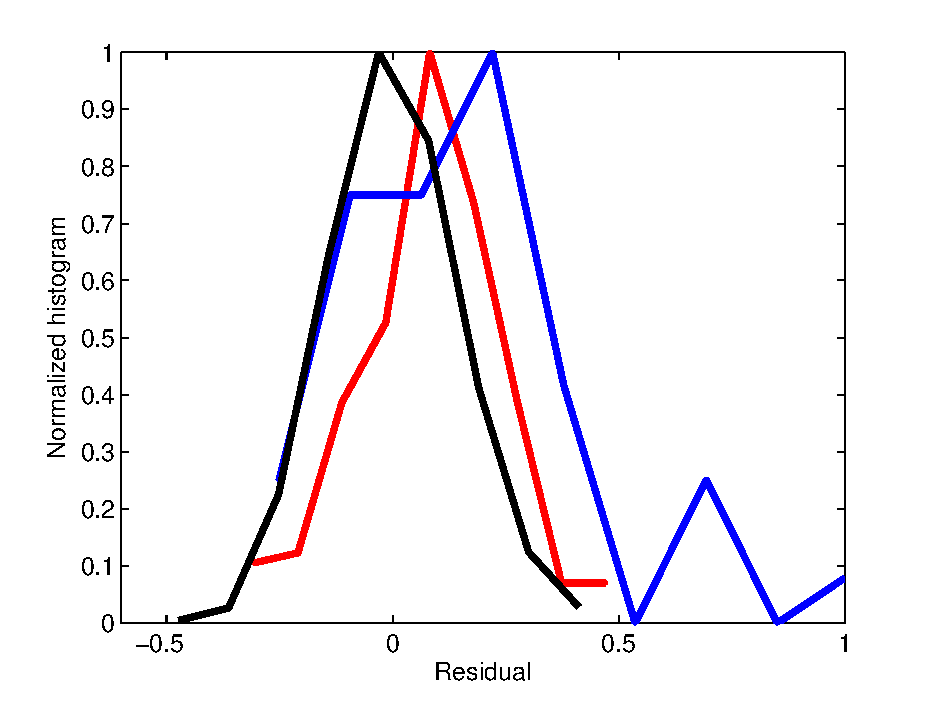
\includegraphics[width=\hsize]{../figs/Figure10a_residuals_iidglm}
\end{minipage}
\begin{minipage}[c]{0.30\hsize}
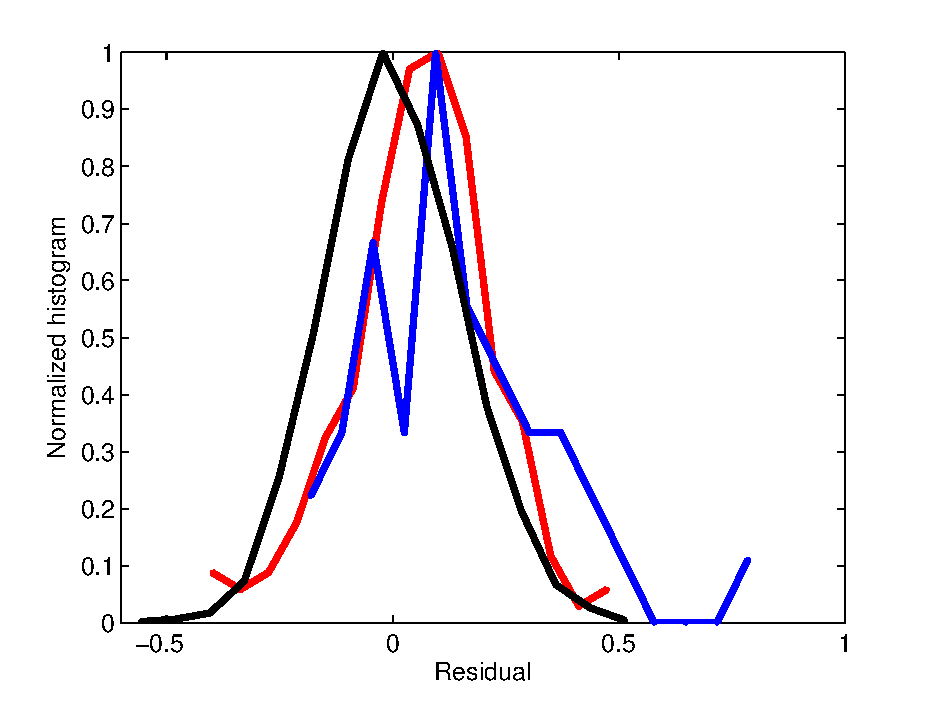
\includegraphics[width=\hsize]{../figs/Figure10b_residuals_baseglm}
\end{minipage}
\begin{minipage}[c]{0.30\hsize}
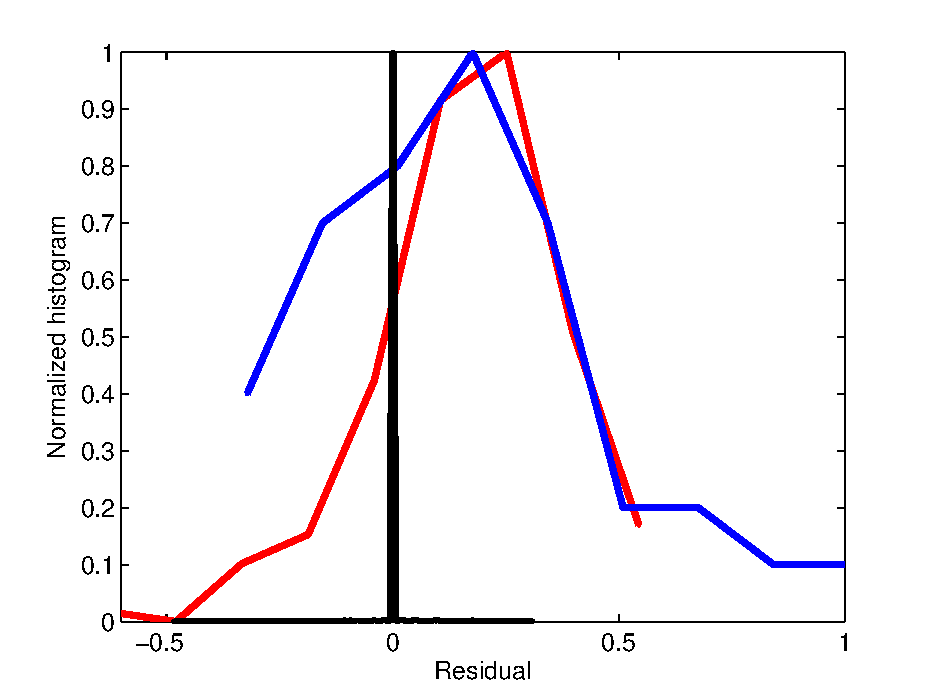
\includegraphics[width=\hsize]{../figs/Figure10c_residuals_basespa}
\end{minipage}
\caption{Normalized histograms of residual errors in the inferred connectivity weights, for
a network of $N=50$ neurons and $T=800$ s. The inferred distributions were rescaled
to have the same mean with the true distributions, owing the time-discretization scaling bias
discussed in the text.
Left panel is for independent approximation using regular GLM, middle panel is
for baseline regular GLM solution, and the right panel is for baseline
sparse GLM solution.}
\label{fig:residuals}
\end{figure}

\begin{figure}[h]
	\centering
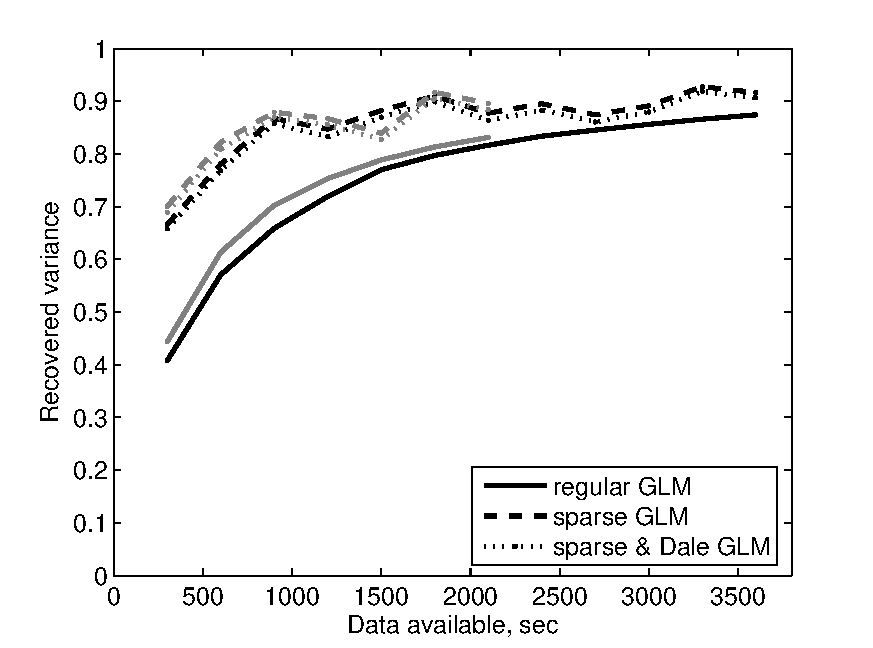
\includegraphics[width=250pt]{../figs/Figure4_perf_vs_T}
\caption{Baseline accuracy of connectivity weights inference as the function of imaging time. Black lines are for $N=50$ and gray lines are for $N=100$. Note that accuracy does not depend on the number of neurons $N$, as shown in the Methods. Also, about 30 minutes of imaging time are sufficient for accurate estimation of the connectivity matrix using GLM solution, while the same accuracy of the reconstruction may be achieved with sparse-prior GLM solver already for 300-600 seconds of calcium imaging.}
\label{fig:data-time}
\end{figure}

\begin{figure}[h]
	\centering
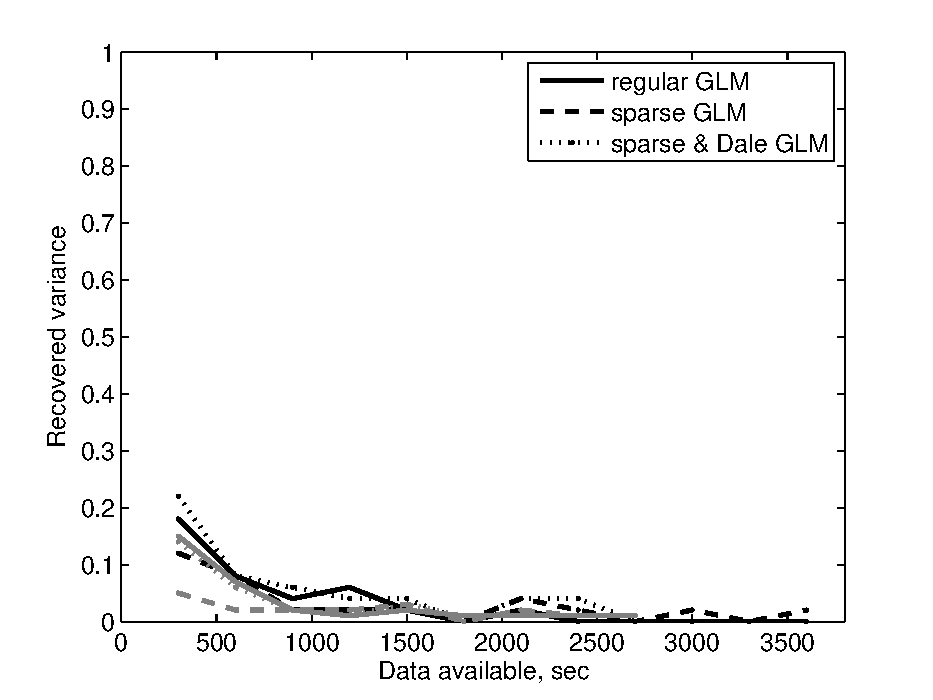
\includegraphics[width=250pt]{../figs/Figure11_inhexc_errors}
\caption{Baseline accuracy of the inferred neuron type (excitatory or inhibitory) as the function of imaging time. Black lines are for $N=50$ and gray lines are for $N=100$. Better than 95\% accuracy
is achieved in identification of neuron type.}
\label{fig:data-ie}
\end{figure}